\documentclass[conference]{IEEEtran}
\IEEEoverridecommandlockouts
% The preceding line is only needed to identify funding in the first footnote. If that is unneeded, please comment it out.
\usepackage{cite}
\usepackage{amsmath,amssymb,amsfonts}
\usepackage{algorithmic}
\usepackage{graphicx}
\usepackage{textcomp}
\usepackage{xcolor}
\def\BibTeX{{\rm B\kern-.05em{\sc i\kern-.025em b}\kern-.08em
    T\kern-.1667em\lower.7ex\hbox{E}\kern-.125emX}}
\begin{document}

\title{Defining an Interface for Autonomous Vehicle Steering Software\\
%{\footnotesize \textsuperscript{*}Note: Sub-titles are not captured in Xplore and
%should not be used}
%\thanks{Identify applicable funding agency here. If none, delete this.}
}

\author{\IEEEauthorblockN{1\textsuperscript{st} Given Name Surname}
\IEEEauthorblockA{\textit{dept. name of organization (of Aff.)} \\
\textit{name of organization (of Aff.)}\\
City, Country \\
email address or ORCID}
\and
\IEEEauthorblockN{2\textsuperscript{nd} Given Name Surname}
\IEEEauthorblockA{\textit{dept. name of organization (of Aff.)} \\
\textit{name of organization (of Aff.)}\\
City, Country \\
email address or ORCID}
}
\maketitle

% Outline
% Discuss the problem of software reusability and safety verification in autonomous driving
% Discuss whether waypoints should be output by high-level autonomous driving algorithms 
% Discuss waypoints vs corridor/maneuver representation with more freedom but less software reusability
% Discuss existing algorithms, corridor, PID w/ genetic algorithm optimization, complex path-tracking (MPC) ,our code
% Discuss their benefits from a reusability perspective
% somewhere we should discuss electronic stability and how it is already embedded into low level control / ECU
% Discuss the need for better evaluation of actual algorithm performance (leaving the opportunity open for a new paper!)


\begin{abstract}
%This and the IEEEtran.cls file define the components of your paper [title, text, heads, etc.]. %*CRITICAL: Do Not Use Symbols, Special Characters, Footnotes, 
%or Math in Paper Title or Abstract.
TODO: write abstract. % TODO
\end{abstract}

\begin{IEEEkeywords}
autonomous driving, steering controller, mpc, optimal control,
\end{IEEEkeywords}





\section*{Introduction}

Advanced driver assistance systems (ADAS) and autonomous vehicles are a rapidly growing segment of the automotive industry. In 2004, Audi researchers reported that software advances accounted for 80\% of innovations in new vehicles \cite{softwarereuse2004}. Since then, the prevalence of ADAS and autonomous driving has rapidly increased.
%(TODO: discuss how the industry has grown - figures from this week's ME 302b presentation.)

The rise of automotive software presents new challenges in software reusability. To equip more vehicles with autonomous software, manufacturers must be able to develop autonomous driving stacks for vehicles with different capabilities and sensor configurations, verify safety-critical software, and comply with numerous regulations and standards. Software reuse is a key component of this process, enabling rapid development of autonomous driving for different vehicle platforms.

Some portions of the software, such as route planning, object recognition, and other high-level decision-making processes, are hardware-agnostic. However, lower-level software such as steering and acceleration control is more dependent on the vehicle's specific hardware. To optimize fuel efficiency, for example, a gasoline-powered vehicle must be driven differently than an electric-gas hybrid or fully electric vehicle with regenerative braking. Tire-road interactions, vehicle dynamics, engine performance, and other mechanical characteristics inform this optimization. Clearly, this part of the autonomy stack is much less portable between different vehicles.


\section*{Steering and Acceleration for Autonomous Vehicles}

Major concerns with steering and acceleration control for autonomous vehicles include fuel efficiency, passenger comfort, and safety. However, different applications of autonomy put different weight on these objectives. An autonomous truck delivering cargo would prioritize fuel efficiency, but may not carry any passengers. An autonomous taxi must avoid making maneuvers that would cause discomfort or alarm to customers. Many ADAS-equipped vehicles on the market today offer the option of switching between ``sport" and ``eco-friendly" modes, which change the driving behavior of the car, raising the possibility that fully autonomous consumer vehicles would offer the same type of configurable experience. % TODO: Citation needed?)

\subsection*{Software Reusability Considerations}
Given the hardware dependencies of low-level control software, an initial idea to tackle software reusability may be to minimize the amount of software being written. One could seek to make the division between hardware-agnostic and hardware-specific software as far ``down" the stack as possible to maximize software reuse. However, this presents issues in practice. Suppose our high-level software plans driving maneuvers (such as turning, stopping, holding a certain speed or distance from another vehicle) and decomposes these maneuvers into a trajectory of closely spaced waypoints that specify the vehicle's state over time. Then the low level controller must only track this trajectory, assuming it is correct. Unfortunately, without hardware information the vehicle will follow a sub-optimal path. In dynamic maneuvers such as emergency braking, this could become dangerous.

\subsection*{Performance Considerations}
A more performant approach is to divide the software when driving maneuvers are specified. The low-level controller would be provided data about these maneuvers, such as the road boundaries and specific, desired states (stopping at a at a stop sign, keeping a safe distance behind another car). The specific trajectory taken to execute these maneuvers is then computed by the low-level controller, using hardware-specific information to optimize the trajectory. For example, a hybrid with regenerative braking can recover electric energy, while a vehicle without this capability may spend more time coasting to a stop and less time actively braking. A vehicle that is aware its tires could slip can steer more conservatively. However, the optimizing controller is coupled to the hardware. The performance benefit must be weighed against the development cost of these vehicle-specific controllers.

\subsection*{Trajectory Tracking vs Optimization} Are waypoints the best representation of the vehicle's path? A higher-level representation, such as the road boundaries and obstacles, allows the steering controller to determine its own trajectory but is more difficult to develop and verify. In this paper we explore the question of tracking vs optimization by discussing the implementation of an optimizing controller.


\section{Implementations of Steering and Acceleration Controllers}
Many steering and acceleration controllers have been developed for varying purposes. We focus on examples of specific categories: classical control, and optimal control (such as model-predictive control (MPC)). Most of these examples are tracking controllers: the objective is to follow a reference trajectory as closely as possible.

\subsection{Classical Control for Trajectory Tracking}
PID controllers can be applied to steering and acceleration control; however, tuning the PID gains remains challenging. Mohajer et al. define a multi-objective problem to evaluate a trajectory for efficiency and passenger comfort, then apply a genetic algorithm to optimize their controller's PID gains offline \cite{pid}. This significantly reduced path tracking error and undesirable high-frequency control inputs over their baseline of hand-tuned PID gains. Information about the vehicle's hardware is required to complete the PID tuning. The authors use 28 numerical parameters describing the vehicle's geometry, inertia matrices, and shock absorber performance to simulate the PID controller during the optimization process. This suggests in a practical application, the tuning procedure would need to be rerun if, for example, the vehicle is loaded with heavy cargo. Alternatively, PID gains could be pre-computed for a variety of different configurations.


Classical control has also been applied to more complex vehicle models. Chebly et al. develop a multi-body model of the vehicle using robotics methods, using 21 bodies connected by joints to  represent the vehicle's chassis, suspension, steering, and wheels.  \cite{CHEBLY201712526} This model uses 12 parameters including vehicle mass, inertia, and cornering stiffnesses of tires. The high fidelity of this vehicle model enables the design of a steering and acceleration controller that successfully tracks a reference trajectory across a wide range of driving conditions and performs well in highly nonlinear situations \cite{CHEBLY201712526}. The authors also discusses the controller's robustness to errors caused by variations in the vehicle's mass or tire stiffness, verifying the controller can continue to track the reference trajectory in with a $\pm30\%$ error in these parameters.

\subsection{MPC Trajectory Tracking}
Farag et al. apply MPC for trajectory tracking to achieve high performance driving around ``complex" tracks featuring tight curves and hairpin turns \cite{farag}. Notably,
this performance is achieved with only two parameters listed: the distances $l_f$ and $l_r$ from the vehicle's center of mass to its front and rear wheels, respectively. This is achieved by using a simple kinematic bicycle model for the vehicle. The authors note that this increases the algorithm's portability to different vehicles.

The use of few physical parameters appears in several other MPC algorithms. Daoud et al. develop  a dual-objective nonlinear MPC formulation for trajectory tracking, allowing an electric vehicle to switch between ``sport" and ``eco-friendly" driving modes. This algorithm uses the kinematic bicycle model with an additional simplification: the center of gravity (CG) is assumed to be at the center of the wheelbase, so only one parameter is needed: the wheelbase length $l$. The front and rear axles are then a distance $l/2$ away from the CG. An additional parameter describes the efficiency of the electric motor. 


\subsection{Trajectory Optimization}


There are fewer optimizing controllers, likely due to the increased difficulty of design. One paper on this topic applies an inner model control framework to the problem of path tracking: computing an optimal trajectory and controlling the vehicle to follow it \cite{pathtracking}. The road is represented as a corridor of allowable space. The authors note that due to the added complexity of accurate nonlinear vehicle models, their controller uses the simplified bicycle model (with three parameters: mass, and the two distances between the CG and front/rear axles). They also use a linear approximation to model tire forces, with two additional parameters for front and rear tire stiffness.

In this algorithm, the path tracking problem is split in two parts. First, given a road corridor where it is safe to drive, a trajectory is selected from the space of possible trajectories in the corridor. An optimal control input is computed. The authors then design an inner model controller driven by this signal to account for disturbances in the vehicle \cite{pathtracking}.


\section{Practical Considerations}

Many considerations inform the selection of a vehicle model, including nonlinearity, accuracy in extreme situations such as emergency maneuvers with high steering curvature and acceleration, ease of computation (particularly for optimal controllers such as MPC), and ease of system identification. Additional practical concerns include the controller's robustness against inaccurate or changing parameters.

In real life, disturbances such as passengers, heavy cargo and fuel can perturb the vehicle's weight and CG. Weather and temperature effects can change the tire performance. A practically applicable controller must be robust against inaccuracies in its vehicle  model. Alternatively, the controller could implement an online estimation method to update parameters, allowing a high standard of performance to be maintained under changing configurations.

\section{Implementation of a Nonlinear MPC Trajectory Optimizer}

To study the challenges and benefits associated with optimizing controllers, we implemented one using nonlinear MPC (NMPC). The controller used a simple kinematic bicycle model for the vehicle, shown in Figure \ref{fig:kinematic}. This is the same model used in \cite{farag} with $n=4$ state variables, $m=2$ control signals, and two system parameters: $l_f$, the distance from the center of mass (CoM) to the front axle, and $l_r$, the distance from the CoM to the rear axle.

\begin{figure}[htbp]
	\centering
	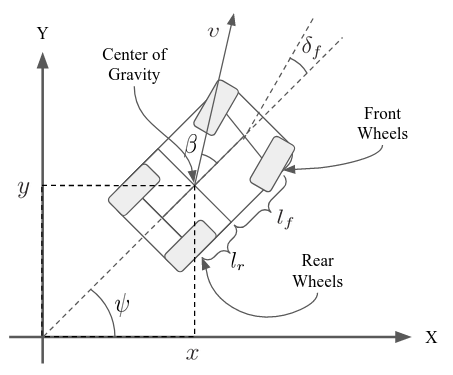
\includegraphics[width=0.8\linewidth]{kinematic_diagram.png}
	\caption{Kinematic bicycle model.}
	\label{fig:kinematic}
\end{figure}

\begin{equation}
z = \begin{bmatrix}
x\\y\\v\\\psi
\end{bmatrix},\quad \begin{bmatrix}
\dot x\\\dot y\\\dot v\\\dot\psi
\end{bmatrix} = \begin{bmatrix}
v\cos(\psi + \beta)\\
v\sin(\psi + \beta)\\
a\\
\frac{v}{l_r}\sin(\beta)
\end{bmatrix}
\label{eq:kinematic}
\end{equation}
where $\beta$, the angle between the car velocity and its longitudinal axis, is defined in  \eqref{eq:beta}. The state vector is $z \in \mathbb{R}^4$.

\begin{equation}
\beta = \tan^{-1}\Big( \frac{l_r}{l_f + l_r}\tan(\delta_f) \Big)
\label{eq:beta}
\end{equation}

The control signals are $a$, the longitudinal acceleration of the car, and $\delta_f$, the steering angle of its front wheels. The control vector is $u = [a\ \delta_f]\ \in \mathbb{R}^2$.

We consider an NMPC problem with lookahead steps $k=1,\dots,N$ spaced a distance $\Delta_t$ apart. The nonlinearity is confined to the dynamics model \eqref{eq:kinematic}. The cost function is quadratic and the state and control constraints are all representable by linear inequalities.

The problem is initialized with the initial vehicle state and a desired speed for each lookahead step $v_{des,1},\dots,v_{des,N}$. Obviously, the desired speed should not vary much over the lookahead distance.

Taking inspiration from a paper in which a ``driveable corridor" is defined \cite{li6640152}, allowing the optimization algorithm to choose the vehicle's path within the corridor, we used a list of linear inequalities to represent the road as shown in Figure \ref{fig:roadpolygons}. Each right and left boundary corresponds to one step: if there are $N$ lookahead steps, $2N$ lines must be generated.

\begin{figure}[h]
	\centering
	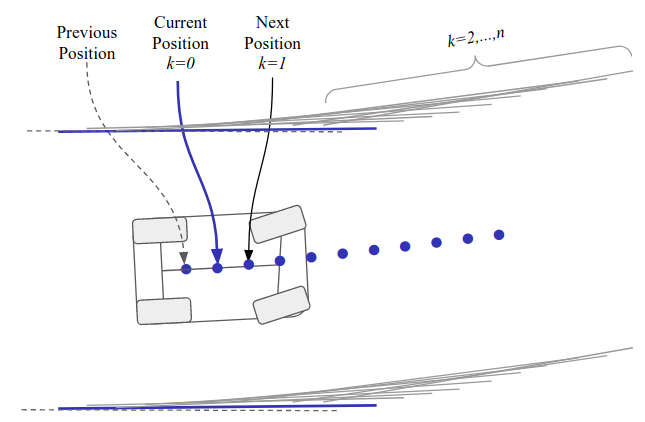
\includegraphics[width=0.9\linewidth]{road_final_bounds.png}
	\caption{A short sample of overlapping lines to define the road corridor. 2 lines are used per step: for an MPC problem with steps $x_1,\dots,x_N$, $2N$ lines are required.}
	\label{fig:roadpolygons}
\end{figure}

This representation was selected to simplify the optimization problem. At each step, the allowable $x-y$ position of the vehicle can be represented by a set of linear inequalities. By generating a new polygon for each lookahead step, arbitrarily tight curvatures can be represented by decreasing the time between each step. In our implementation, four-sided polygons are used to simplify software development.

The cost function contains terms to penalize sharp turns and acceleration, which degrade passenger comfort, and to penalize deviations from the center of each polygon (otherwise the vehicle may drive close to the boundaries of the road, which is confusing to other drivers and alarming to passengers).

The cost terms are:

\begin{equation}
J_{accuracy} = \sum_{k=1}^N\big\| \begin{bmatrix}
x_k\\y_k\\\psi_k
\end{bmatrix} - \begin{bmatrix}
x_{center,k}\\y_{center,k}\\\psi_{center,k}
\end{bmatrix} \big\|_2^2
\label{eq:costcenter}
\end{equation}
where $(x_{center,k}, y_{center,k}. \psi_{center,k}$ describe the $x-y$ position and angle of the center of the $k$th polygon.

\begin{equation}
J_{speed} = \sum_{k=1}^N (v_k - v_{des,k})^2
\label{eq:speed}
\end{equation}
The cost terms in \eqref{eq:costcenter} and \eqref{eq:speed} are separated so they can be weighted differently. Equation \eqref{eq:costcenter} controls the accuracy of the path-following behavior, while \eqref{eq:speed} controls how closely the vehicle stays at the desired speed.


Equations \eqref{eq:costjerk} and \eqref{eq:coststeering} penalize undesirable sharp changes in acceleration and steering angle.

\begin{equation}
J_{jerk} = \sum_{k=2}^N (a_k - a_{k-1})^2
\label{eq:costjerk}
\end{equation}

\begin{equation}
J_{steering} = \sum_{k=2}^N (\delta_{f,k} - \delta_{f,k-1})^2
\label{eq:coststeering}
\end{equation}

By separating these terms, they can be weighted to produce different behaviors as shown in \eqref{eq:costfinal}.
\begin{equation}
J = a_1 J_{accuracy} + a_2 J_{speed} + a_3 J_{jerk} + a_4 J_{steering}
\label{eq:costfinal}
\end{equation}

The final NMPC problem is:
\begin{align}
\text{minimize}\quad& J(z_1,\dots,z_N, u_1,\dots,u_N)
\\
\text{subject to} \quad& z_{k} = f(z_{k-1}, u_{k-1}),\ k=1,\dots,N
\\
& u_{min} \leq u_k \leq u_{max},\ k=1,\dots,N
\\
& \begin{bmatrix}
v_{min}\\\psi_{min}
\end{bmatrix} \leq \begin{bmatrix}
v_k\\\psi_k
\end{bmatrix}\leq \begin{bmatrix}
v_{max}\\\psi_{max}
\end{bmatrix},\ k=1,\dots,N
\\
&
A_k\begin{bmatrix}
x_k\\y_k\\
\end{bmatrix} \geq 0,\ k=1,\dots,N
\end{align}
where $A_k$ is a matrix of linear inequalities that describe the road boundaries at the $k$th step.


We use the bold $\textbf{z} = z_1,\dots,z_N$ and $\textbf{u} = u_1,\dots,u_N$ to denote a full trajectory of $N$ steps. The final algorithm is then:
\begin{algorithmic}
\REQUIRE $z_0,\ v_{min},\ v_{max},\ u_{min},\ u_{max}$,\texttt{weights}\\\COMMENT{Weights for cost function \eqref{eq:costfinal}.}
\STATE $z \leftarrow z_0$
\\
\WHILE \TRUE
\STATE $\textbf{v}_{des} \leftarrow$ \texttt{get\_desired\_speed(}$z$\texttt{)}
\STATE $A_1,\dots,A_N\leftarrow $  \texttt{generate\_road(}$z,\ \textbf{v}_{des}$\texttt{)}
\STATE \texttt{bounds} = $(A_1,\dots,A_N,\ v_{min},\ v_{max},\ u_{min},\ u_{max})$
\STATE $\textbf{z},\ \textbf{u}\leftarrow$ \texttt{solve\_nmpc(}$z_0$\texttt{, bounds, weights)}
\STATE $z \leftarrow f(z, \textbf{u}_1)$
\ENDWHILE
\end{algorithmic}


\subsection{Implementation Details}

The control limits are given in \eqref{eq:controllimits}. Because the $x-y$ position of the vehicle will be constrained by the linear inequalities, there is no need to impose any other condition on it. The velocity was constrained to $[0, 50.0\ m/s]$.

\begin{equation}
\begin{bmatrix}
-5\\-\pi/4
\end{bmatrix} \leq \begin{bmatrix}
a\\\delta_f
\end{bmatrix} \leq \begin{bmatrix}
2.5\\\pi/4
\end{bmatrix}
\label{eq:controllimits}
\end{equation}

The problem was defined using CasADi in Python and solved with ipopt \cite{Casadi} \cite{ipopt}. Ipopt requires initialization when solving a nonlinear optimization problem: a rough guess of speed and position must be provided. To reduce computation, the initial guess for the $k+1$th NMPC problem is computed using the solution of the $k$th problem, % TODO: more details on this?
This provided a significant speedup.

\section{Results}
Figure \ref{fig:isolanechange} shows the road as described by the polygon boundaries. Though each boundary is rectangular, they overlap to produce an accurate representation of the road.

Figures \ref{fig:steering_low} and \ref{fig:errors} show the steering angle signal and position error computed by the nonlinear MPC for several sets of weights given in Table \ref{tab:weights}. In this test the simulated vehicle navigates the ISO double lane-change path (Figure \ref{fig:isolanechange}). The initial speed provided to the optimizing controller was 10 $m/s$.

The error can be evaluated several ways: Because the desired velocity was constant ($10 m/s$), the velocity error can be seen in Figure \ref{fig:velocity_low}.

The position error \eqref{eq:poserror} measures the distance of each x-y position $(x_k, y_k),\,k=1,\dots,N$ from the center of its polygonal bound. This is the same measurement used in the cost function \eqref{eq:costcenter}.
\begin{equation}
\text{Position error} = 
\Big\|\begin{bmatrix}x_k\\y_k\end{bmatrix} - \begin{bmatrix}x_{center,k}\\y_{center,k}\end{bmatrix}\Big\|_2
\label{eq:poserror}
\end{equation}

\begin{figure}[htbp]
	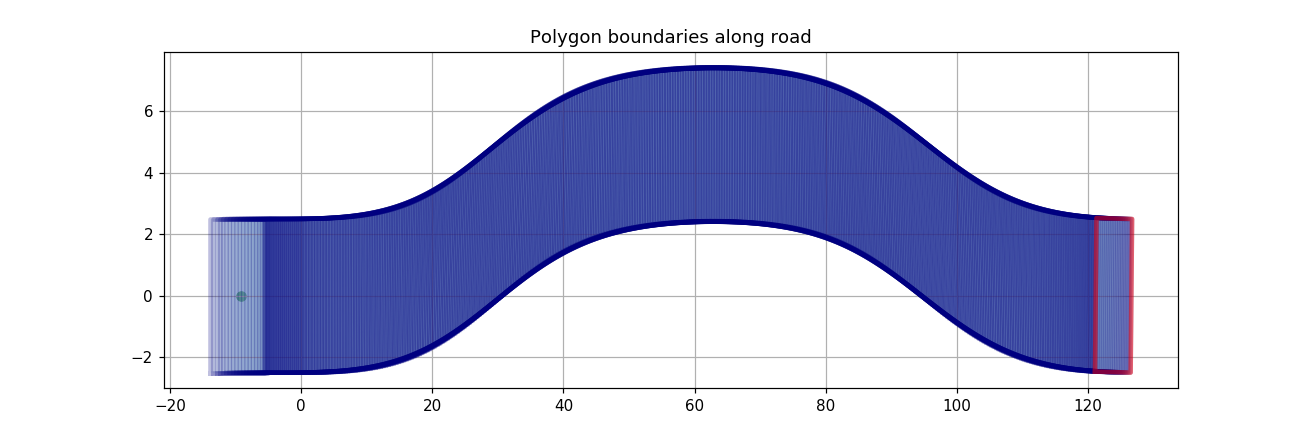
\includegraphics[width=1.0\linewidth]{polygon_bounds_iso_lanechange.png}
	\caption{Polygon boundaries describing the ISO double lane change path. The path has a width of 5 meters.}
	\label{fig:isolanechange}
\end{figure}

%\begin{figure}[htbp]
%	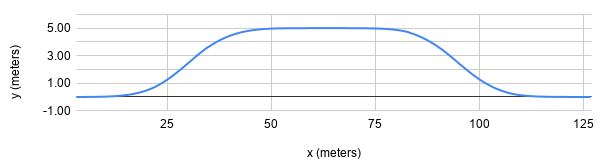
\includegraphics[width=1.0\linewidth]{iso_lanechange_matches_data.png}
%	\caption{The center of the ISO lane-change road}
%	\label{fig:isocenter}
%\end{figure}

\begin{figure}[tbp]
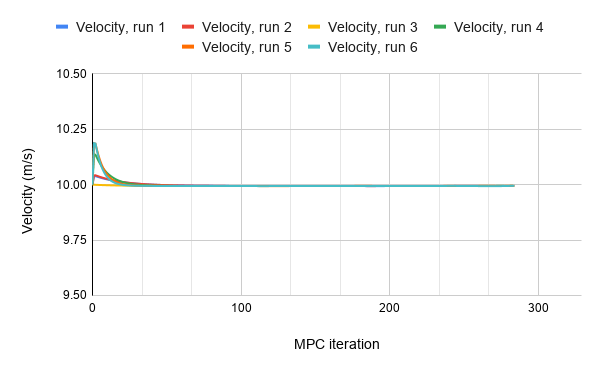
\includegraphics[width=1.0\linewidth]{velocity.png}
\caption{Velocity profile (desired speed is 10 m/s). There is some initialization difficulty, likely due to the issue shown in Figure \ref{fig:centering_error}  when  generating the first set of road center points. Once this error is overcome, the vehicle stays almost exactly at the desired speed.}
\label{fig:velocity_low}
\end{figure}\

\begin{figure}[tbp]
	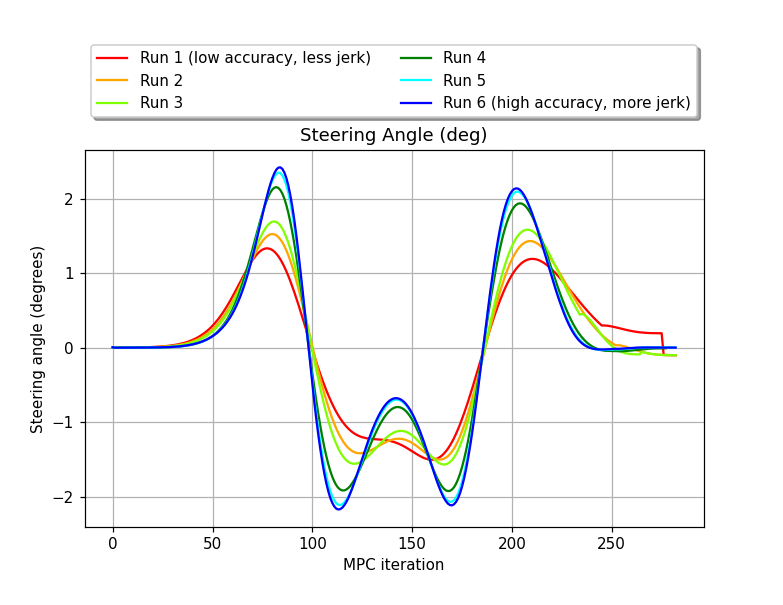
\includegraphics[width=1.0\linewidth]{steering_angle.png}
	\caption{Steering angle control signal for a low-speed test (desired velocity is 10 m/s).}
	\label{fig:steering_low}
\end{figure}

\begin{figure}[htbp]
	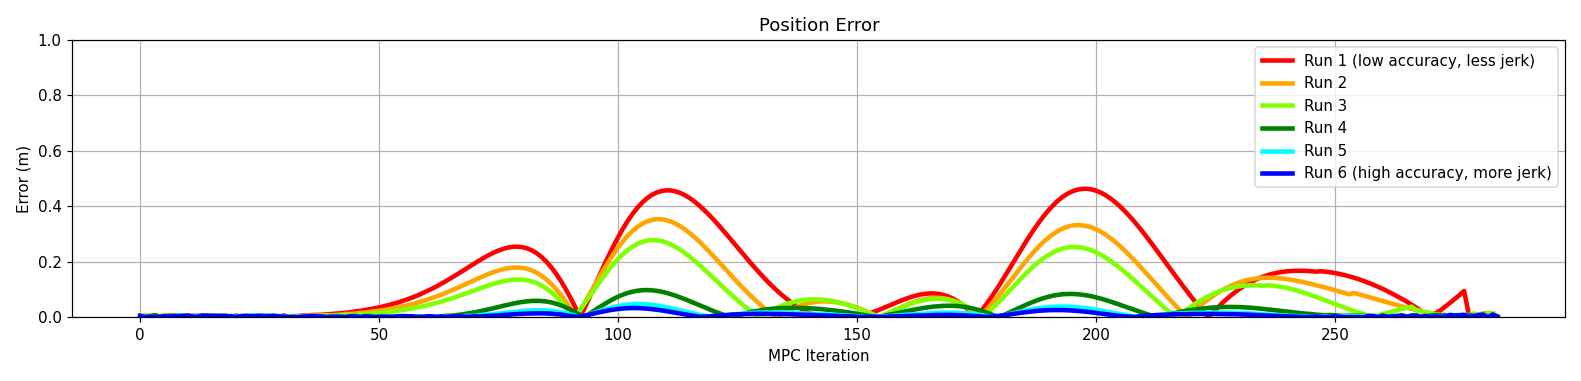
\includegraphics[width=1.0\linewidth]{errors.png}
	\caption{Position error \eqref{eq:poserror}. Runs with less weight on accuracy \eqref{eq:costcenter} had higher error but required smaller control inputs as shown in Figure \ref{fig:steering_low}.}
	\label{fig:errors}
\end{figure}

As expected by the weights in Table \ref{tab:weights}, increasing the cost associated with the jerk (change in acceleration) and change in steering angle produces a smoother velocity profile and smoother control signals.
$$J = \textcolor{red}{\alpha} J_{accuracy} + 10\textcolor{red}{\alpha} J_{speed} + 100 J_{jerk} + 10\frac{180}{\pi} J_{steering}$$

\begin{table}[htbp]
	\caption{Cost weights for \eqref{eq:costfinal} used in the MPC simulations. The weights of \eqref{eq:speed} and \eqref{eq:costjerk} are increased to produce increased smoothing of the vehicle trajectory.}
	\centering
	\renewcommand{\arraystretch}{1.25}
	\begin{tabular}{c|cccccc}
		Run & 1 & 2 & 3 & 4 & 5 & 6
		\\\hline
		$\alpha$ & 0.01 & 0.05 & 0.1 & 1.0 & 5.0 & 10.0
		%\\
		%$J_{speed}$ & 0.1 & 0.5 & 1.0 & 10.0 & 50.0 & 100.0
	\end{tabular}
\label{tab:weights}
\end{table}

\subsection{Changing Vehicle Parameters}
The kinematic bicycle model used in this paper has 2 parameters, $l_r$ and $l_f$, describing the vehicle CG with respect to the front and rear axles. To study the effects of parameter changes on the controller output, we moved the CG forwards and backwards, as might occur in a vehicle transporting heavy cargo.

All runs were computed with cost weights corresponding to the ``mid-range" performance of the previous section:
$$J = 0.1J_{accuracy} + J_{speed} + 100J_{jerk} + 10\frac{180}{\pi} J_{steering}.$$
Ideally, the accuracy and control signals should be similar since the same cost function is being applied.

Figures \ref{fig:velocity_low_cg}, \ref{fig:steering_low_cg}, and \ref{fig:errors_cg} show these expected results. With the CG moved forward or back, the vehicle becomes less maneuverable. The speed lowers slightly from the initial estimate of 10 $m/s$. 

\begin{figure}[h!]
	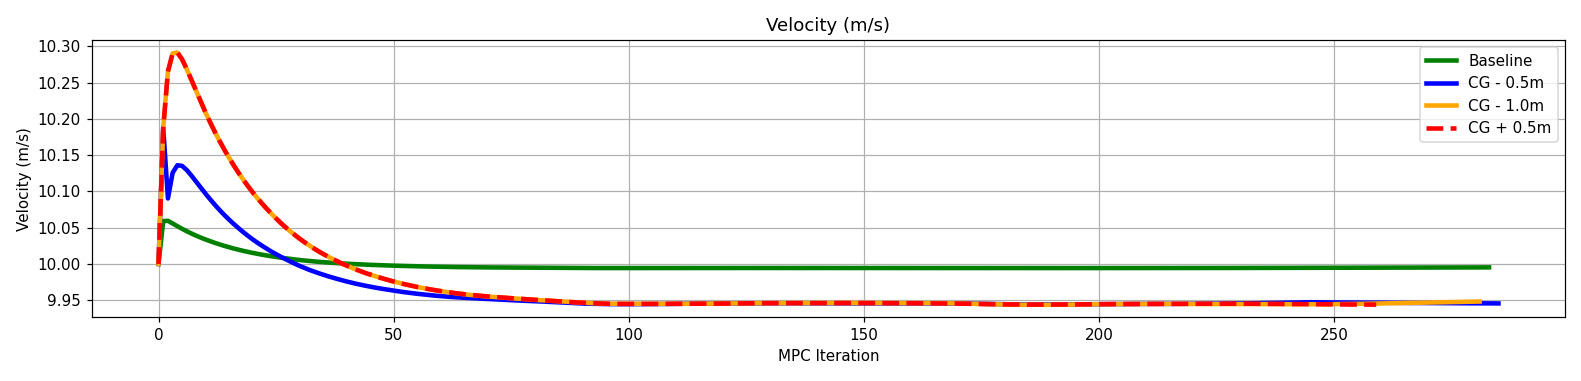
\includegraphics[width=1.0\linewidth]{velocity_cg.png}
	\caption{Velocity profile (desired velocity is 10 m/s). There is some initialization difficulty, likely due to the issue shown in Figure \ref{fig:centering_error}  when  generating the first set of road center points. The optimizing controller decreases the velocity slightly when the CG moves forwards or back.}
	\label{fig:velocity_low_cg}
\end{figure}\

\begin{figure}[h!]
	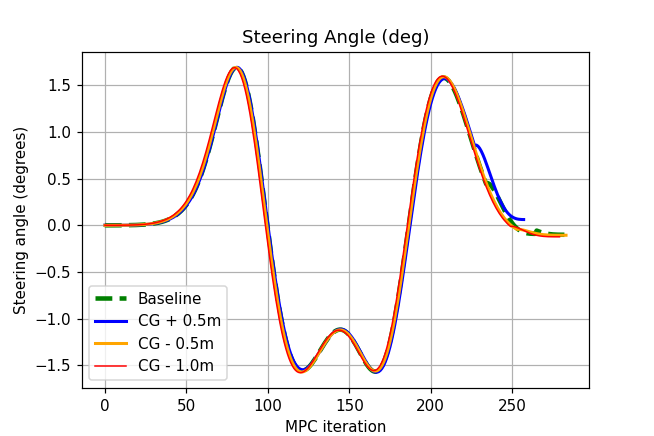
\includegraphics[width=1.0\linewidth]{steering_angle_cg.png}
	\caption{Steering angle control signal with varying CG. The control signals are very similar, likely because the cost function weights were not changed.}
	\label{fig:steering_low_cg}
\end{figure}

\begin{figure}[h!]
	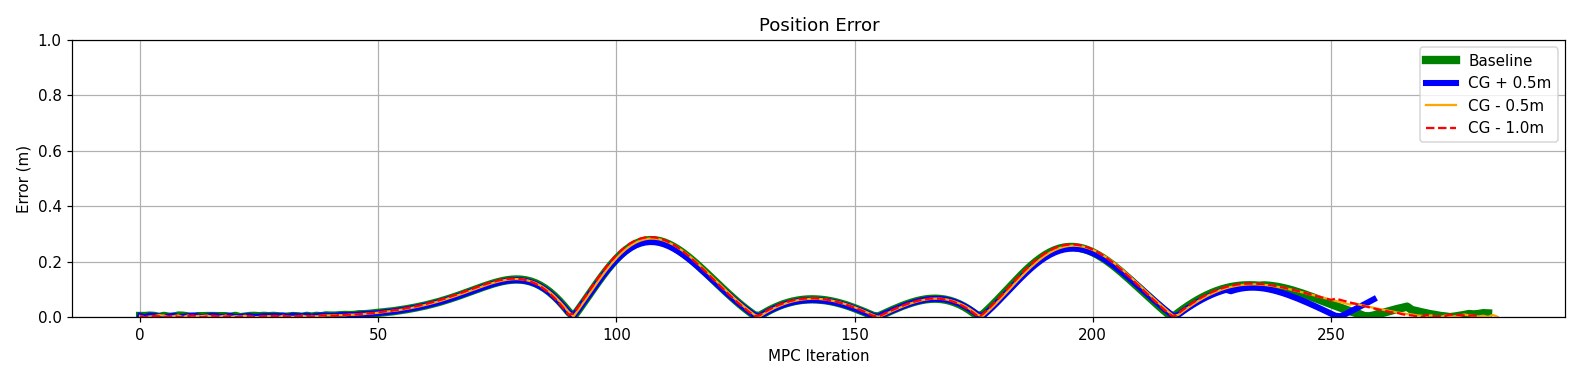
\includegraphics[width=1.0\linewidth]{errors_cg.png}
	\caption{Position error \eqref{eq:poserror} with varying CG. The error is very similar, likely because the cost function weights were not changed..}
	\label{fig:errors_cg}
\end{figure}

%\footnote{The original direct collocation code was provided with CasADi and can be found at \texttt{https://github.com/casadi/casadi/blob/
%		master/docs/examples/python/direct\_collocation.py}}.
	
	
	
	
	
\label{sub:impl}
\subsection{Implementation Difficulties}

The primary implementation difficulties encountered while programming the NMPC controller were related to road representation: the problem of converting numerical data representing the road (such as a list of center points and road widths) to a mathematically useful format. Other papers apply a variety of methods: fitting polynomials, Bezier curves, or other smooth functions to the data. We chose to represent the road center and width using Bezier curves.
Unfortunately, in trajectory optimization the vehicle can stray from the center curve if it provides better performance on other metrics (such as reducing jerk and steering angle). This complicates the  cost function.

%The road representation should have the following properties:

%The road should be smooth; if its curvature changes suddenly, this induces undesirable sudden changes in steering and acceleration.

%Additionally, the vehicle should be able to travel on arbitrarily long roads. There should be some way to continuously stitch new points to the road representation. (We did not implement this. Though it is mathematically possible, for example by generating Bezier curves with constraints on the initial and final curvature (to match previous curves), a software library to do so could not be found.)

%For our NMPC controller, the road object must be able to measure distance between two points on the center curve. This is required for generating the polygonal boundaries used in the MPC code: assuming the vehicle is at position $x_0,\ y_0$ and drives at ``close to" the desired speed $v_{des}$, the distance it has traveled at each step $x_k,\ y_k$ is $v_{des,k}\Delta_t k$. Then the road center at step $k$ is $v_{des,k}\Delta_t k$ away from $x_0,\ y_0$.

%However, the vehicle does not stay on the road centerline. To approximate this distance computation, the road object must be able to take an $x-y$ point ``near" the centerline and return the closest point on the centerline.
%This was implemented numerically.

A major issue was formulating a cost function that causes the vehicle to move forward without  unnecessarily penalizing velocity changes.
If the MPC problem is initialized with a (suboptimal) speed estimate, choosing points on the road center for steps $1,\dots,N$ without introducing ``noise" in the accuracy term of the cost function \eqref{eq:costcenter} is difficult (Figure \ref{fig:centering_error}). This issue was resolved by using previously computed trajectories to generate the center points, but is still present in the first MPC iteration.

\vspace{2em}
\begin{figure}[h!]
	\centering
	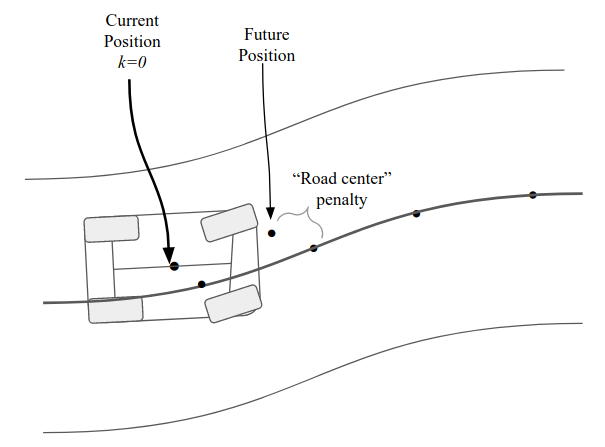
\includegraphics[width=0.9\linewidth]{centering_issue.png}
	\caption{Using poorly chosen center points adds a penalty if the optimal speed deviates from the initial guess.}
	\label{fig:centering_error}
\end{figure}

\subsection{Limitations}
One limitation of the road representation in Fig. \ref{fig:roadpolygons} is that if there is an obstacle in the middle of the road, the vehicle cannot evaluate both paths around it. One must be selected by higher-level software.

%Additionally, the optimized solution cannot deviate far from the desired speed. The desired speed is used to generate the polygonal boundaries, so a large deviation would place the vehicle outside the feasible $x-y$ space. This can be alleviated by using larger polygons, at the expense of precision. Future controllers could adaptively change the polygon size; in a narrow road with high curvature it should be small, while on a highway with high speed and low curvature it could be much larger.

\section{Conclusions}
The controllers discussed in this paper take several approaches to the problem of autonomous vehicle steering. On one side is the question of modeling the vehicle: complex robotics-inspired models can provide more accurate dynamics, but are likely too computationally difficult for an optimal control approach such as MPC. Classical control techniques can be used to analyze these models and design stabilizing controllers as done in \cite{CHEBLY201712526}. Additional concerns include uncertainty and changes in vehicle parameters that could affect the controller's performance in real life, and the difficulty of system identification to port the controller to new vehicle hardware.

Optimal control approaches are also common, but many of them focus on trajectory tracking, which can be achieved via MPC, as opposed to the difficult nonlinear problem of trajectory optimization. New advances in nonlinear MPC may alleviate this issue in the future: more advanced dimensional lifting techniques can approximate the problematic nonlinear dynamics, transforming the problem into a convex quadratic formulation that can be quickly and reliably solved \cite{Korda_2018}.

\section{Future Work}

In this paper, we have discussed the benefits and drawbacks of different steering and acceleration controllers from a hardware portability view. It is difficult to directly compare these controllers because of the lack of standardized tests defined for them. Some researchers select clothoids, commonly used in designing freeway ramps, and Euler spirals to construct test roads \cite{pid}. Others use the roads around their home institution for test data \cite{farag}. One open question is the design of standard driving tests for these controllers. Defining a set of standard paths and vehicle maneuvers for benchmarking controllers will benefit future researchers by enabling easy quantitative comparison of algorithms.

Another avenue of future research is parameter estimation and controller robustness against changing vehicle dynamics. Vehicle mass and CG can change for many reasons: for example, delivery vehicles picking up and dropping off heavy cargo, fuel tanks emptying over a long drive, and trucks transporting liquids that can move in their tanks. To be practically useful, a steering and acceleration controller must be able to adapt as parameters change.
Additionally, some important parameters are difficult to measure and change with road conditions. The parameters describing tire-road interactions cannot be directly measured, but have been estimated using a complex two-step method, accounting for both slow changes (tires degrading over time) and rapid ones (such as driving into a puddle) \cite{GARATTI20091304}. Environmental data such as the road gradient and bank angle are relevant for stability control / anti-rollover systems, but cannot be easily measured: some algorithms exist to estimate them using velocity and engine torque data \cite{mahyuddin2012}. 



%\subsection{Applying Software Standards to Autonomous Steering}
%These standards specify how vehicle software can be architected, but leave open questions in where the division should be made between high-level hardware-independent algorithms and low-level software. One area where this question arises is vehicle steering and acceleration control.

%The task of steering an autonomous vehicle can be divided into software modules for planning the vehicle's route, determining what maneuvers it should make, determining a path to carry out these maneuvers, and generating control inputs to keep the vehicle on the path.

%The question is where this division should be made. Many steering algorithms focus on the path tracking aspect of steering: given a pre-defined path (often a list of waypoints), follow it as closely as possible. Much work has been done on optimizing PID gains, formulating the steering problem using model predictive control (MPC), and other approaches to the path tracking problem. (citations needed).

%\section{Discussion of Steering Software Architecture}
%This paper discusses the pros and cons of two software architecture models for autonomous steering and acceleration.
%% TODO
%\subsection{Division After Trajectory Planning} The split between hardware-specific and hardware-independent software is made after the vehicle's trajectory is determined. This code provides more reusability, since less of it is tied to the vehicle hardware, but does not leave as much room for optimizing the vehicle's trajectory.
%%TODO



%TODO

%\begin{figure}[htbp]
%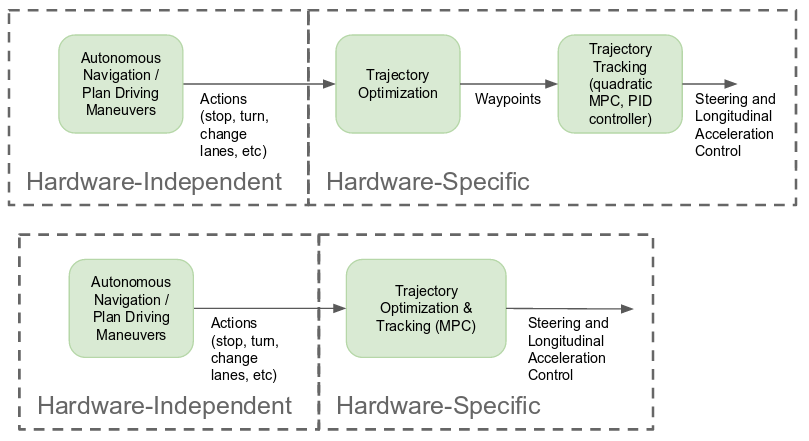
\includegraphics[width=1.0\linewidth]{module_separations.png}
%\caption{Possible software architectures with the proposed division between high and low-level %modules.}
%\label{fig:division}
%\end{figure}


%\subsection{Figures and Tables}
%\paragraph{Positioning Figures and Tables} Place figures and tables at the top and 
%bottom of columns. Avoid placing them in the middle of columns. Large 
%figures and tables may span across both columns. Figure captions should be 
%below the figures; table heads should appear above the tables. Insert 
%figures and tables after they are cited in the text. Use the abbreviation 
%``Fig.~\ref{fig}'', even at the beginning of a sentence.

%\begin{table}[htbp]
%\caption{Table Type Styles}
%\begin{center}
%\begin{tabular}{|c|c|c|c|}
%\hline
%\textbf{Table}&\multicolumn{3}{|c|}{\textbf{Table Column Head}} \\
%\cline{2-4} 
%\textbf{Head} & \textbf{\textit{Table column subhead}}& \textbf{\textit{Subhead}}& \textbf{\textit{Subhead}} \\
%\hline
%copy& More table copy$^{\mathrm{a}}$& &  \\
%\hline
%\multicolumn{4}{l}{$^{\mathrm{a}}$Sample of a Table footnote.}
%\end{tabular}
%\label{tab1}
%\end{center}
%\end{table}

%\begin{figure}[htbp]
%\centerline{\includegraphics{fig1.png}}
%\caption{Example of a figure caption.}
%\label{fig}
%\end{figure}


\section{Acknowledgments}

This work was completed under Professor Sanjay Lall in the Information Systems Lab. The NMPC code was based on several open-source files provided with CasADi.


\bibliographystyle{unsrt}
\bibliography{bibliography}

\end{document}
